\chapter{Test}

%EN 61000-6-2 Immunity standard
%EN 61000-6-3 Emission standard

%\todo[inline]{Remember photos of the different test setups!}
The order of the tests are defined from which tests that can harm the system. The most destructive tests are performed at last. 
\section{Radiation test}
The test is performed in a TEM-cell (Transverse ElectroMagnetic field cell).
The measurement in a TEM-cell can be compared to an open air measurement if the object is small and without inlets. 

\begin{figure}[H]
	\begin{centering}
		 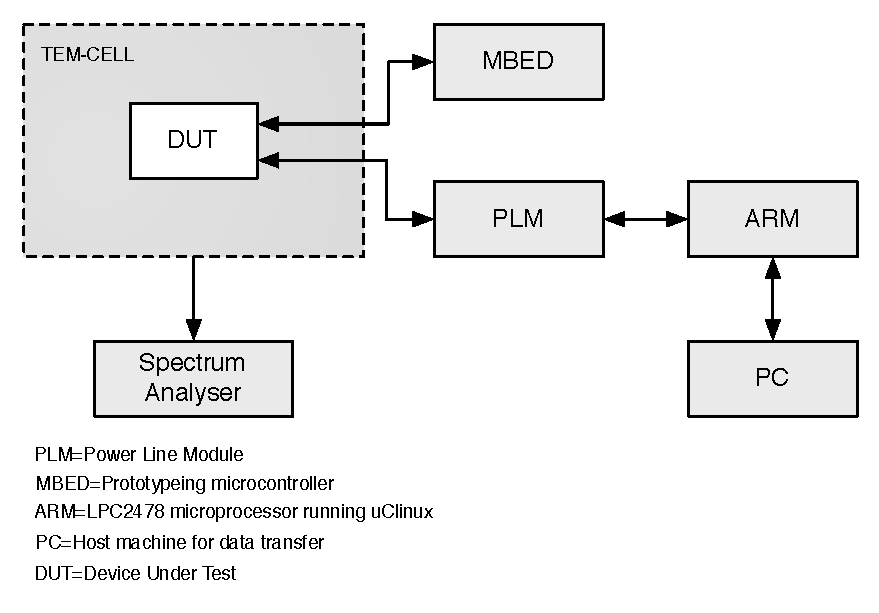
\includegraphics[width=0.8\textwidth]{images/emission_setup.pdf}
		\caption{Emission test setup.}
	\label{fig:emission_setup}
	\end{centering}
\end{figure}
During the test, data was sent from the PC to the ARM board and the Power Supply on the device loaded in order to have the setup to emit the maximum amount of noise. 
\begin{figure}[H]
	\begin{centering}
		 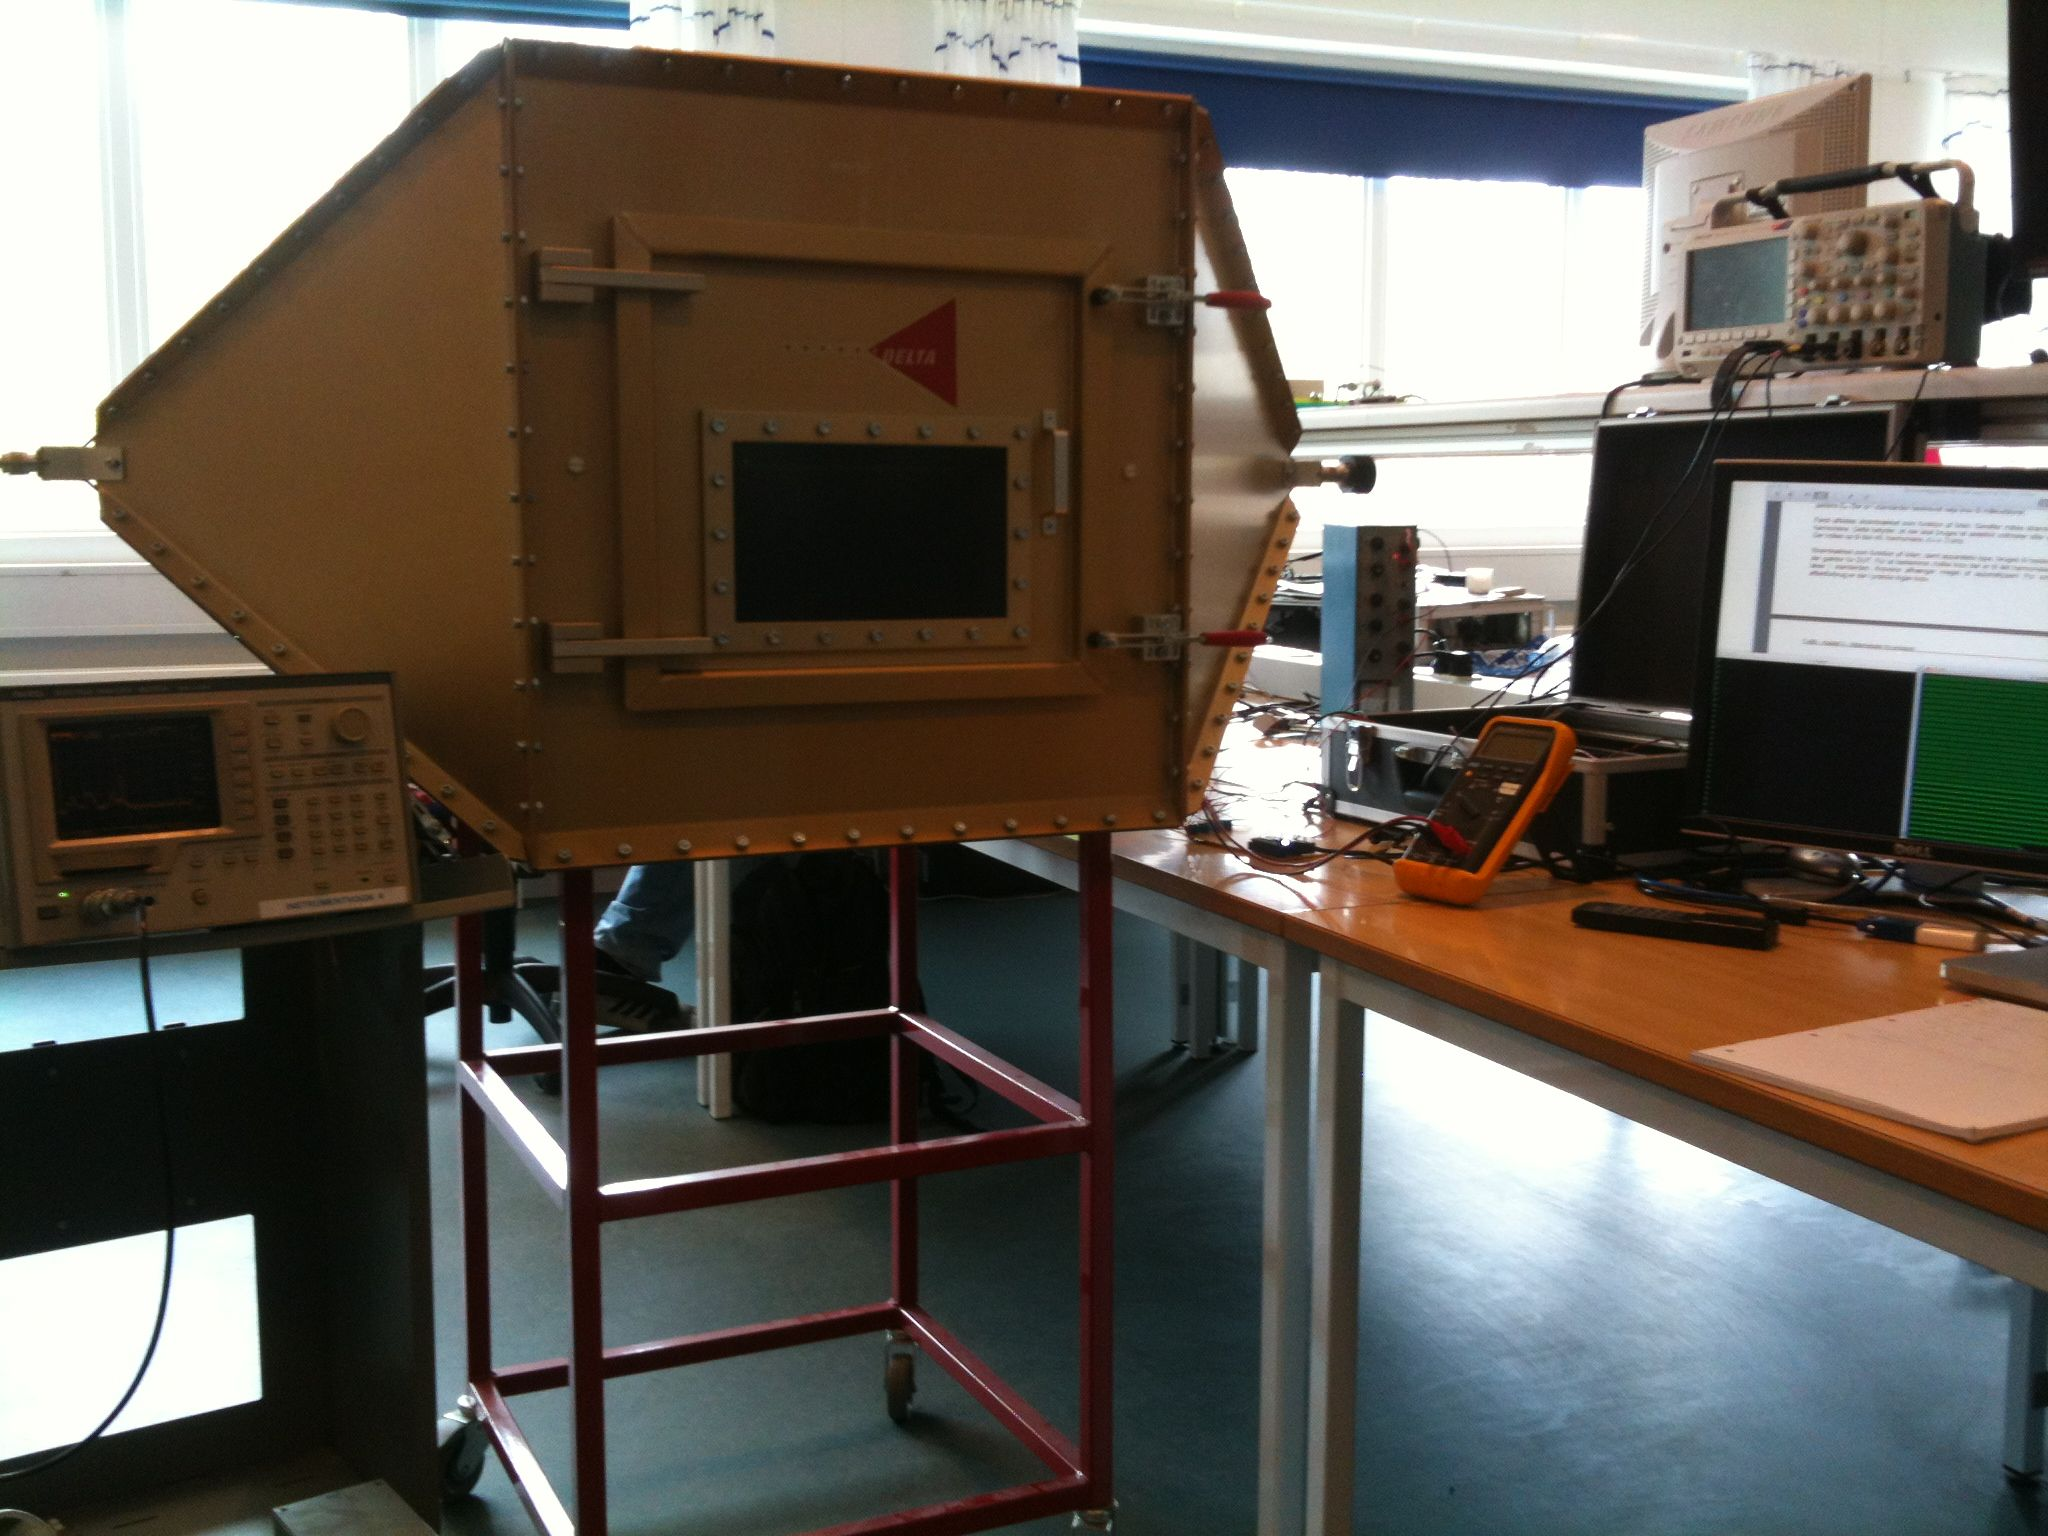
\includegraphics[width=0.8\textwidth]{images/tem_celle_radiation.jpg}
		\caption{Emission test setup.}
	\end{centering}
\end{figure}
The board was rotated in order to find the position where it was emitting its maximum. In picture \ref{fig:board_placement_TEM} the connected board is shown in its maximum emission position. 
\begin{figure}[H]
	\begin{centering}
		 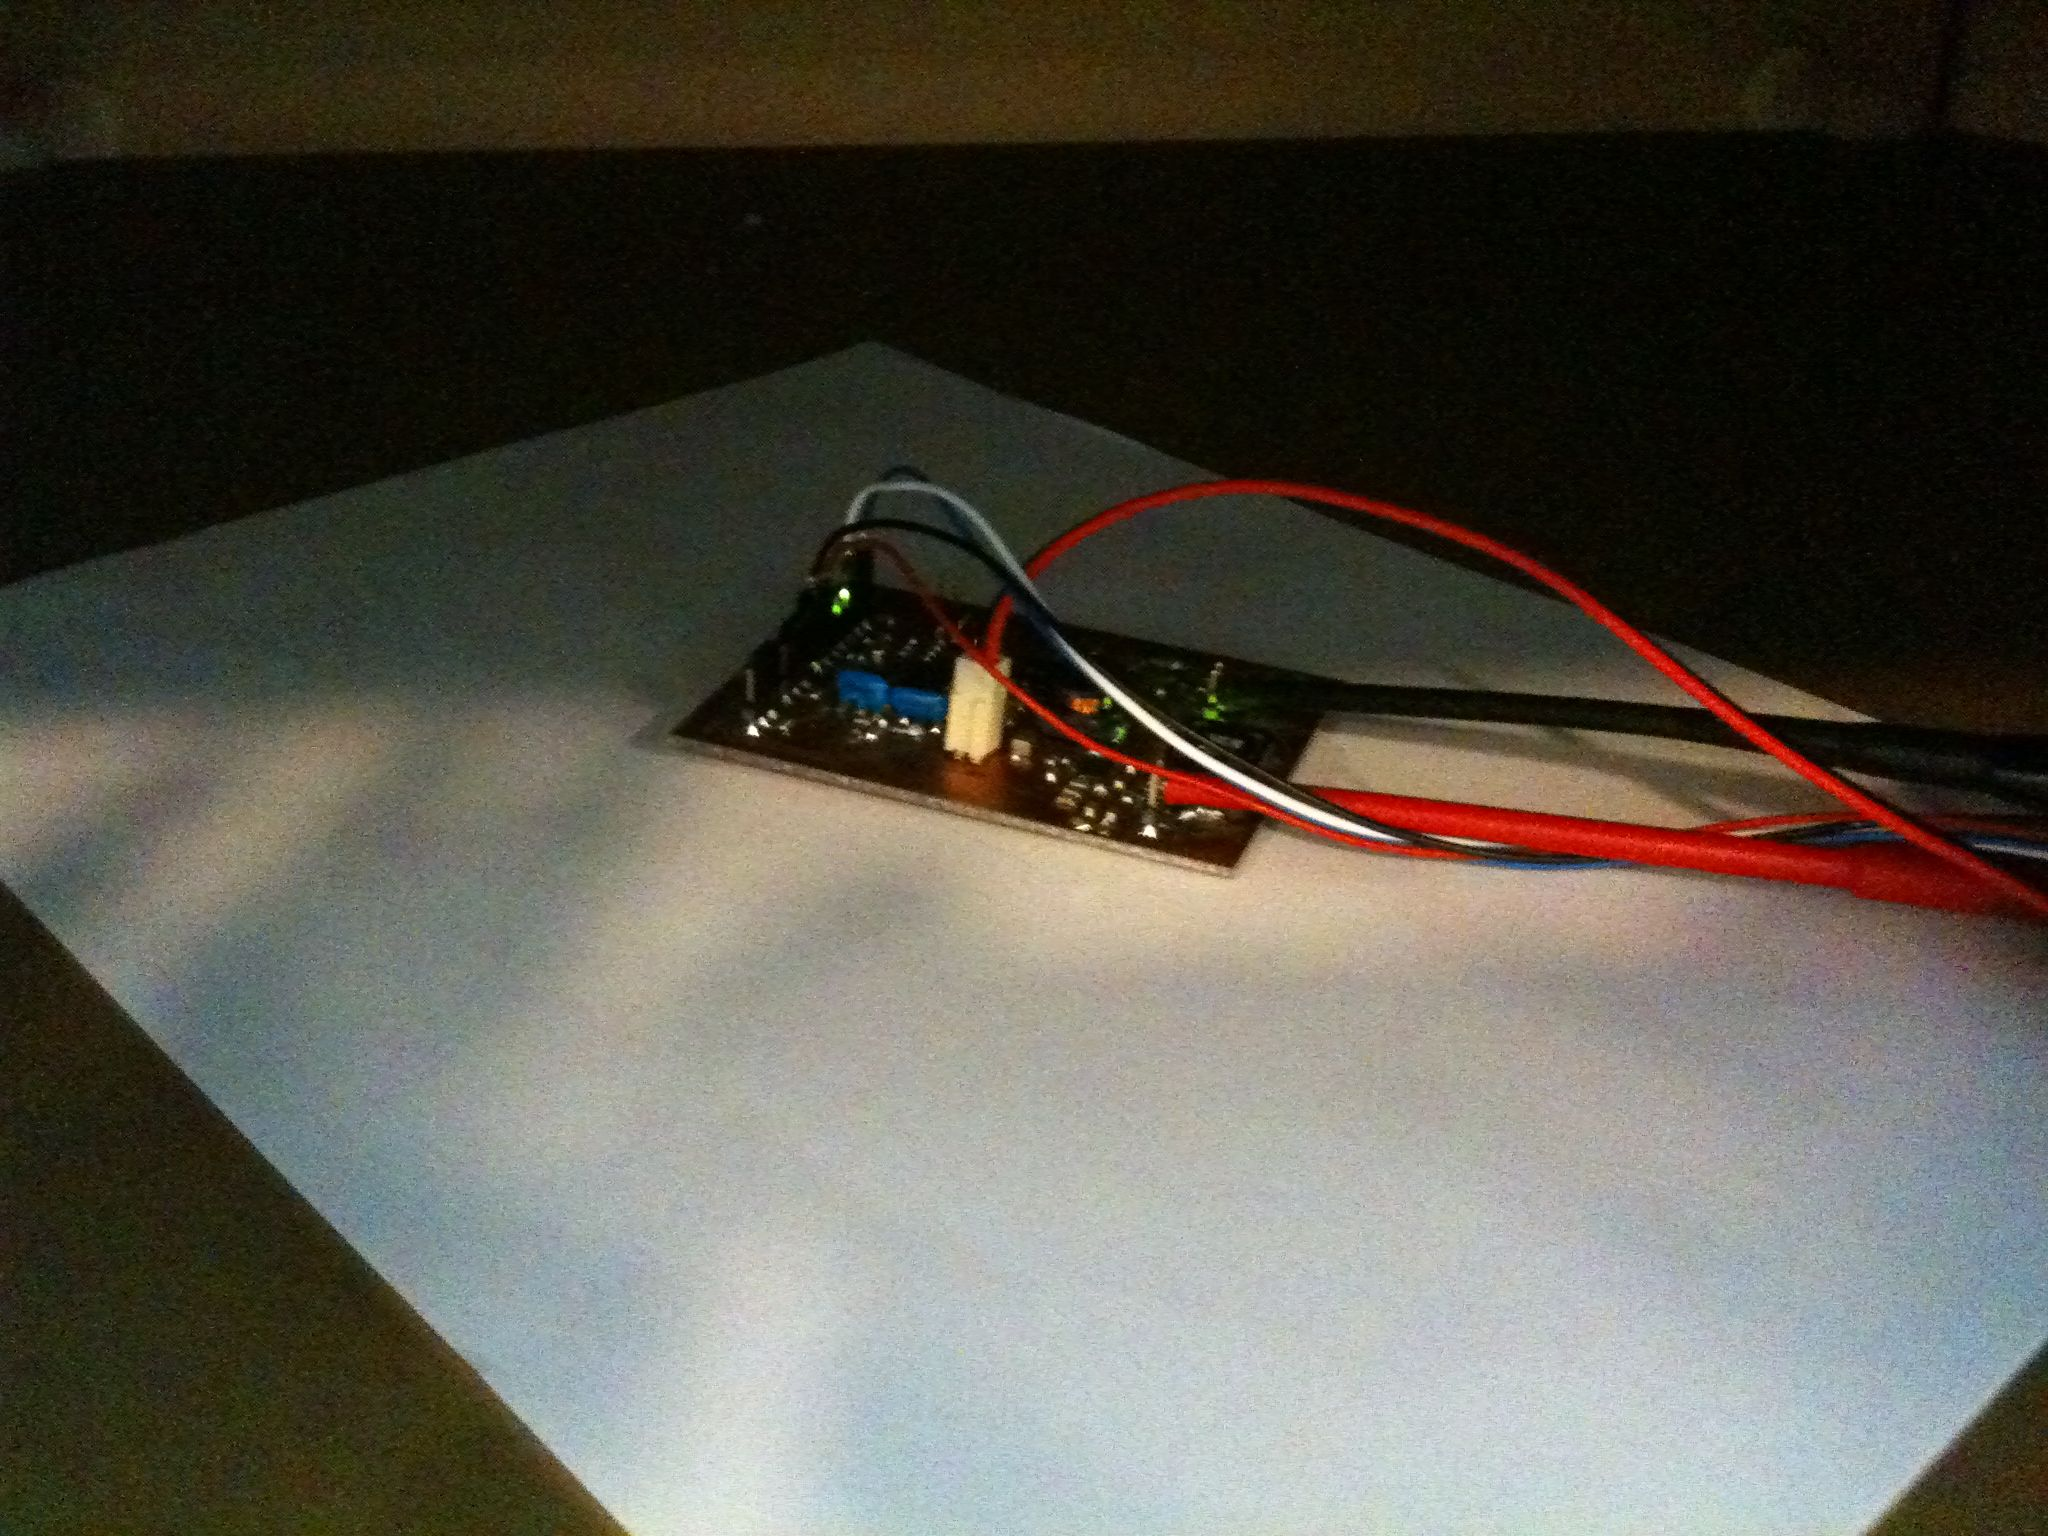
\includegraphics[width=0.6\textwidth]{images/board_placement.jpg}
		\caption{Board placement inside the TEM-cell.}
		\label{fig:board_placement_TEM}
	\end{centering}
\end{figure}
Figure \ref{fig:spectrum_off} shows the spectrum analyzer when the board is turned off. The big spike to the left is the DC level (0Hz).
\begin{figure}[H]
	\begin{centering}
		 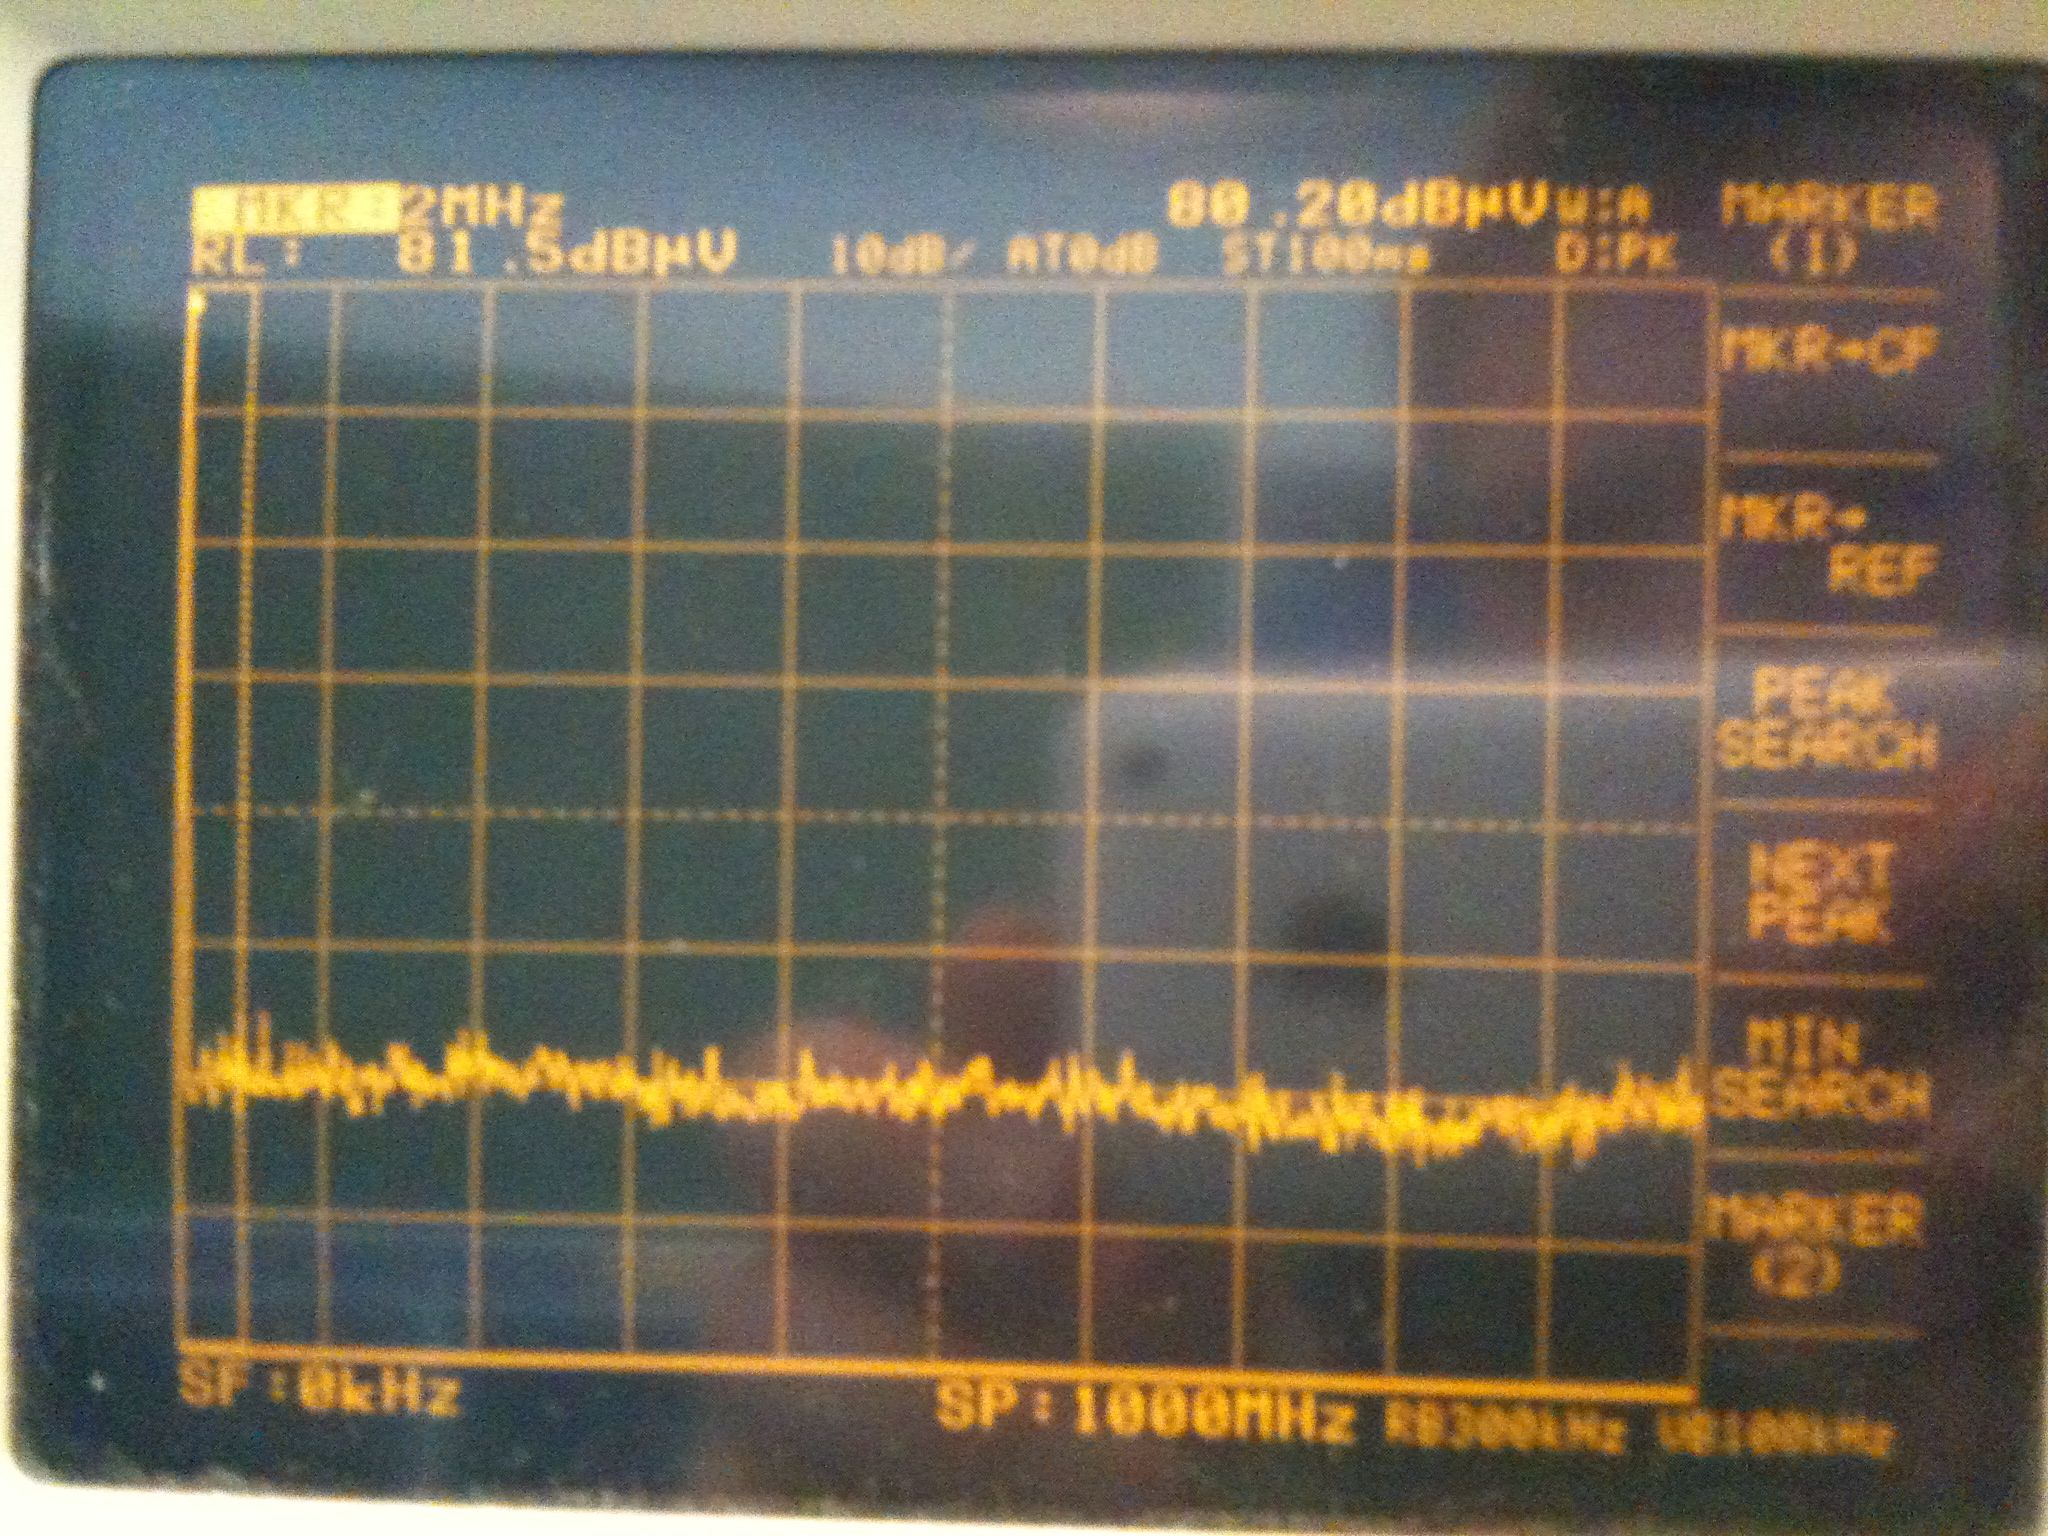
\includegraphics[width=0.6\textwidth]{images/measure_off.jpg}
		\caption{Spectrum analyzer when the device is turned off.}
		\label{fig:spectrum_off}
	\end{centering}
\end{figure}

\begin{figure}[H]
	\begin{centering}
		 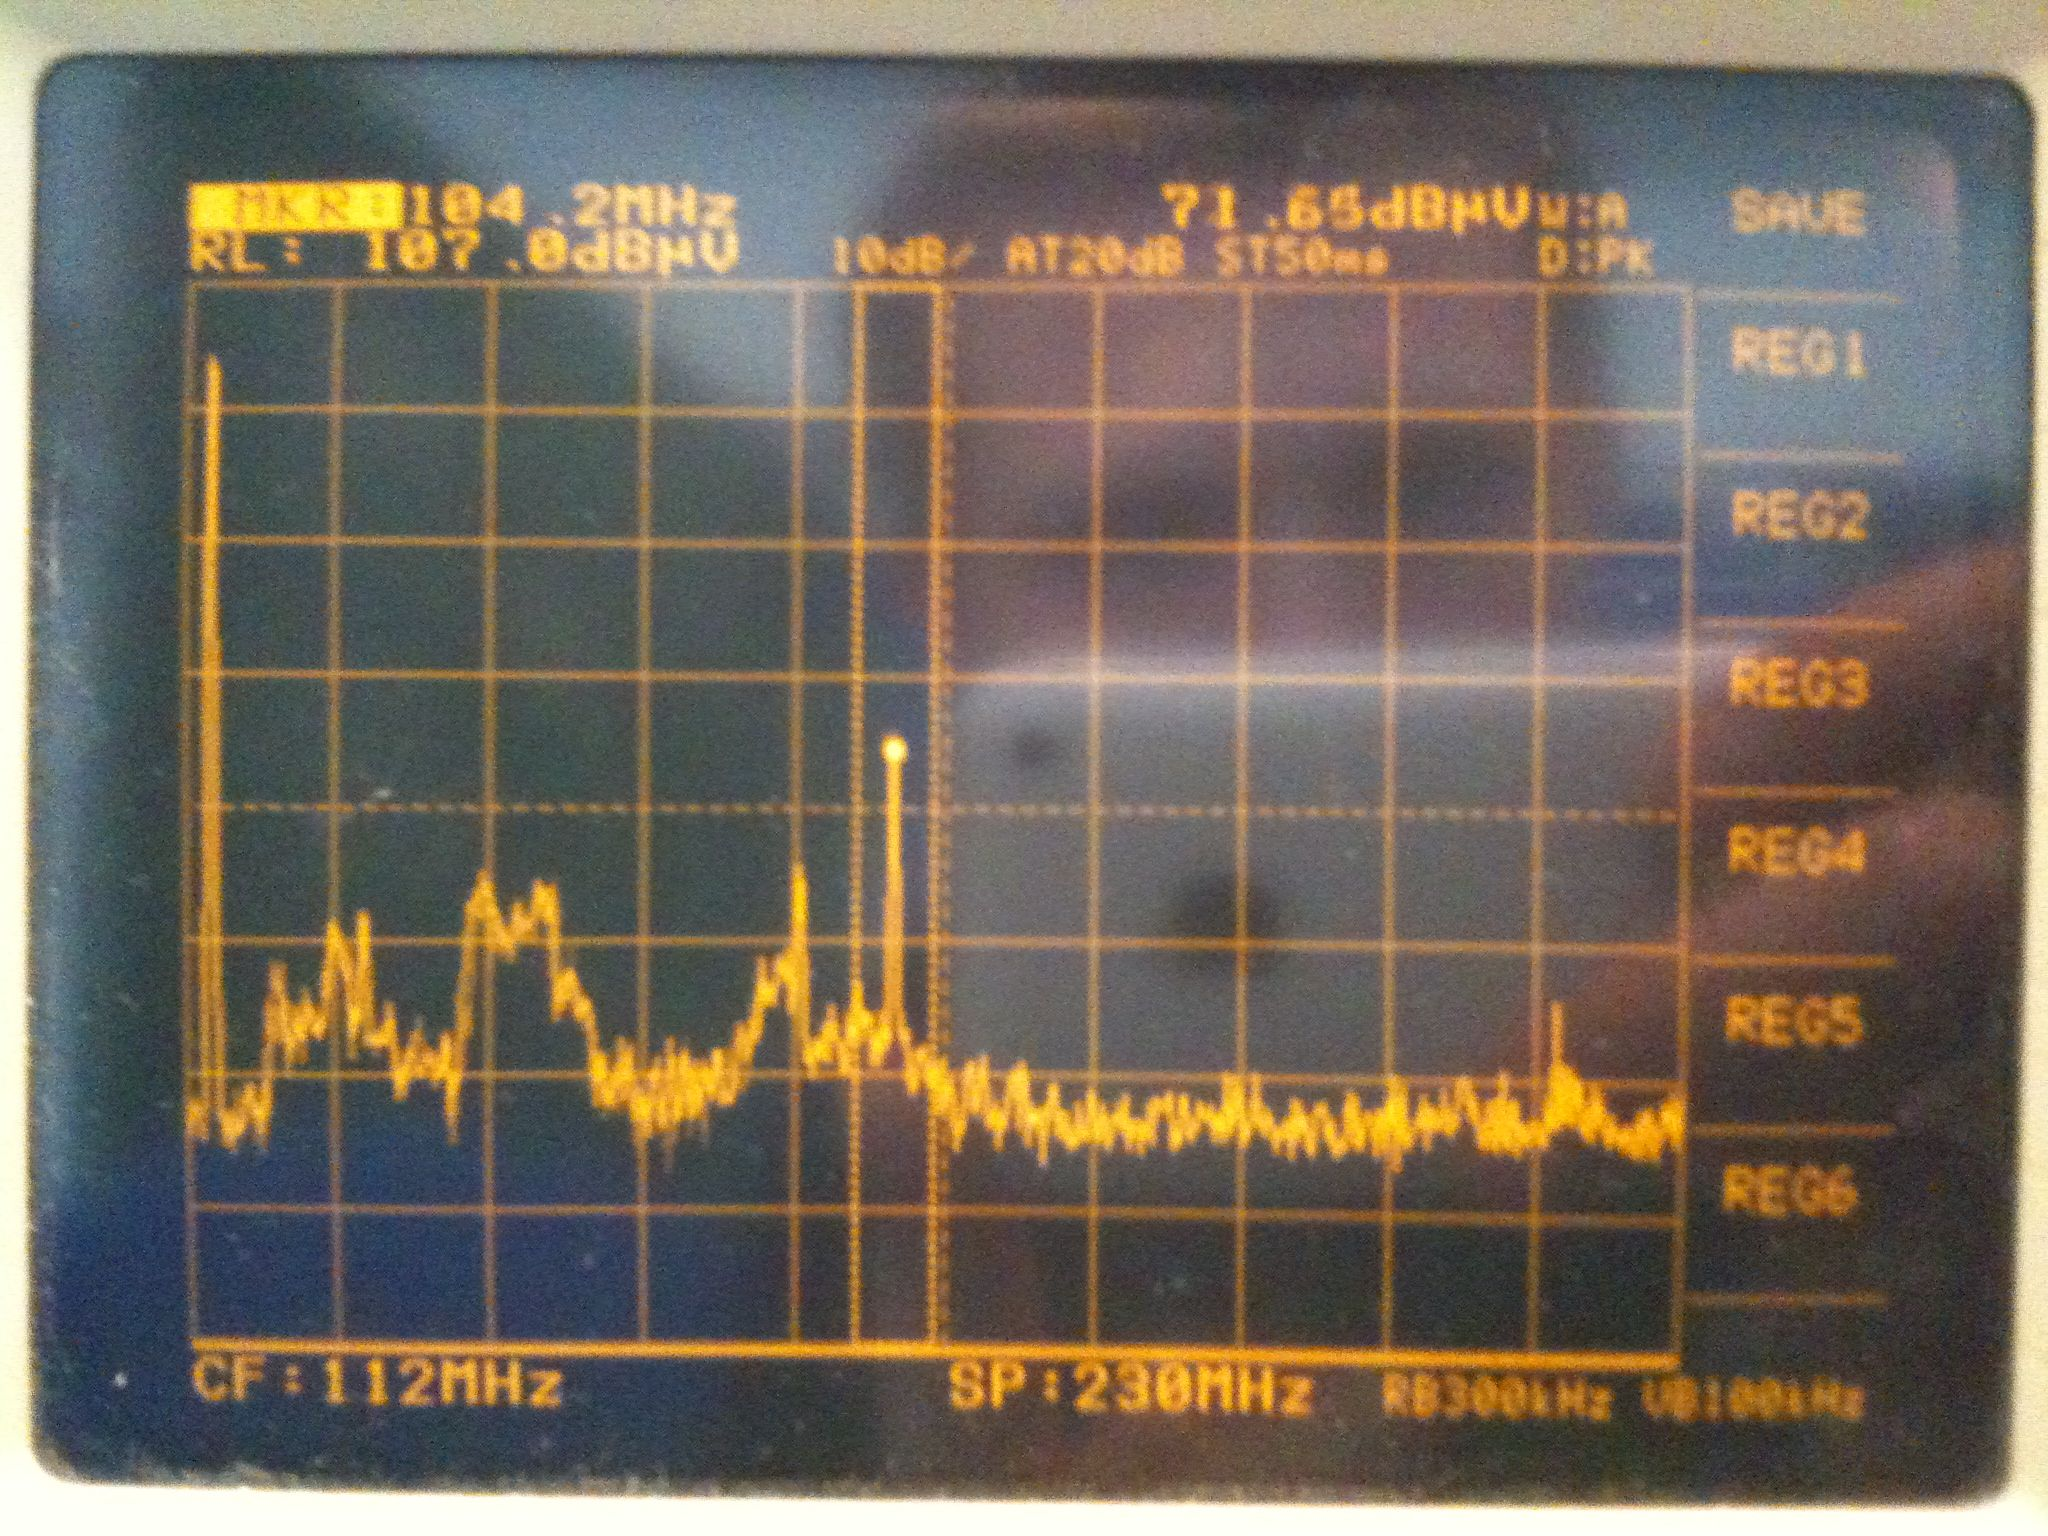
\includegraphics[width=0.8\textwidth]{images/measure_on.jpg}
		\caption{Emission spectrum of the unit. 0 to 230MHz.}
		\label{fig:spectrum_on}
	\end{centering}
\end{figure}
Figure \ref{fig:spectrum_on} shows the maximum level emitted from the device. Note the spike at approximately 100 MHz and the more broad noise at 20 to 50 MHz. Usually spikes comes from microprocessors or similar, in this case the Power Line circuit and the broad noise comes from Switching devices, in this case two switch mode circuits\footnote{Grundlaeggende EMC2 - Page 29}. It is also measured that values above 230MHz are not emitted from the device.
\p The spike at 103MHz is the one emitting the most. As the test are performed in a TEM-Cell, the read value needs to be converted in order to be able to compare to the standards. The conversion is made in a small MathCAD document, fig: \ref{fig:mathcad}
\begin{figure}[H]
	\begin{centering}
		 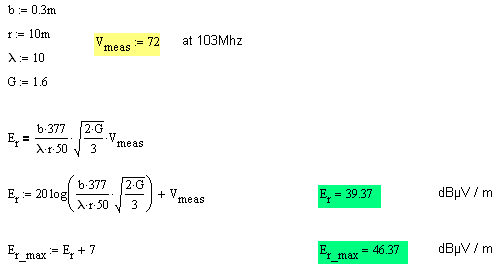
\includegraphics[width=0.8\textwidth]{images/mathcad_emission}
		\caption{MathCAD calculation of the emission.}
	\label{fig:mathcad}
	\end{centering}
\end{figure}
The values read in a TEM-Cell can only be used as guidelines as the offset can be up to 7 dB. This gives a worst case value of $ 46.37 dB\mu V/m$.
\\\p According to table \ref{table:emission_standard_CABINET}\footnote{Table from \textit{Grundleaggende EMC2 - page 73}}, the value measured is approximately $17dB\mu V/m$ higher than the upper limit value.
However, the values from table \ref{table:emission_standard_CABINET} is based on emission limits for cabinet ports. As the device is not mounted in a cabinet, table \ref{table:emission_standard_DC} \& \ref{table:emission_standard_SIGNAL} might be used instead as these describes the emission from the signal and DC ports which is not shielded in this case.
\begin{table}[H]
		\begin{center}
		\begin{tabular}{|l|l|l|l|}\hline
			Fenomena 	& Frequency-span & Limit & Basis standard\\\hline
			~ 			& 30 - 230 MHz		& 30dB($\mu$V/m) in 10 m distance		& CISPR 16-2-3	\\
			~			& 230 - 1000MHz 	& 37 dB($\mu$V/m) in 10 m distance 	& ~				\\\hline
			Radio		& 1 - 3 GHz		& 70 dB($\mu$V/m) peak				& CISPR 16-1-1	\\
			Frequent		&				& 50 dB($\mu$V/m) average			& CISPR 16-1-4	\\
			electro		&				& in 3 m distance					& CISPR 16-2-3	\\
			magnetic		&				& 								& 				\\
			fields		& 3 - 6 GHz		& 74 dB($\mu$V/m) peak				& 				\\
			~			&				& 54 dB($\mu$V/m) average			& 				\\
			~			&				& in 3 m distance					& 				\\\hline
		\end{tabular}
		\end{center}
	\caption{Emission limit  values for cabinet-ports according to the EN 61000-6-3 standard.}
	\label{table:emission_standard_CABINET}
\end{table}

\begin{table}[H]
		\begin{center}
		\begin{tabular}{|l|l|l|l|}\hline
			Fenomena 	& Frequency-span & Limit & Basis standard\\\hline
			Noise		& 0.15 - 0.5 MHz		& 79dB($\mu$V/m) quasi-peak		& CISPR 16-1-2	\\
			~			& ~					& 66dB($\mu$V/m) average		& \& 16-2-1		\\\hline
			Noise		& 0.5 - 30 MHz			& 73dB($\mu$V/m) quasi-peak		& CISPR 16-1-2	\\
			~			& ~					& 60dB($\mu$V/m) average		& \& 16-2-1		\\\hline
		\end{tabular}
		\end{center}
	\caption{Emission limit  values for DC power ports.}
	\label{table:emission_standard_DC}
\end{table}

\begin{table}[H]
		\begin{center}
		\begin{tabular}{|l|l|l|l|}\hline
			Fenomena 	& Frequency-span & Limit & Basis standard\\\hline
			Noise		& 0.15 - 0.5 MHz		& 79-87dB($\mu$V/m) quasi-peak	& CISPR 22	\\
			~ 			& ~					& 84-74dB($\mu$V/m) average	& ~		\\\hline
			Noise		& 0.5 - 30 MHz			& 87dB($\mu$V/m) quasi-peak		& CISPR 22	\\
			~ 			& ~					& 74dB($\mu$V/m) average		& 		\\\hline
		\end{tabular}
		\end{center}
	\caption{Emission limit  values for signal power ports.}
	\label{table:emission_standard_SIGNAL}
\end{table}

In section \ref{sec:design_optimization} (Design Optimization) different suggestions to improving EMC are discussed.

\section{Immunity test}
Down below different test cases are described, which the product has to fulfill in order to be EMC proved and get the CE mark. None of the tests are however performed as the immunity test equipment for the LF magnetic field immunity test and the HF irradiation test is non functional at the time and as the device is a prototype board the ESD and burst / energy transients are not performed. The two last test are not performed as these are meant for a finish product in its housing where the different connectors are stressed in order to verify its immunity. 

\subsection{LF magnetic field immunity \& HF irradiation}
In this section is shortly described how the immunity test for the device shall be performed.
\p The setup for immunity test is equal to the one for emission (see fig: \ref{fig:emission_setup}). During the test the equipment have to fulfill criteria \\A: The equipment have to operate normally during and after the test. \\ By this criteria is in this case meant that the communication have to continue during the test (transmit and receive) and the output voltage have to be kept stabile at its 5 volt level.

\begin{table}[H]
		\begin{center}
		\begin{tabular}{|l|l|l|l|}\hline
			Fenomena 		& Test requirements		& Basis standard 	& Fail criterium	\\\hline
			Radiofrekvent		& 0.15 - 80 MHz		& 				& 			\\
							&					&				&			\\
			CM coubling		& 10 V				& EN 61000-4-6	& A			\\
							&					&				&			\\
			AM modulated		& 80 \% AM (1kHz)		& 				&			\\\hline
		\end{tabular}
		\end{center}
	\caption{Immunity: signal ports and DC power ports}
\end{table}

\subsection{Electrostatic discharge}
Not tested as the board is only in prototype state.

\subsection{Burst and energy transients}
Not tested as the board is only in prototype state.

\section{Design optimization}\label{sec:design_optimization}
As the radiation test did not fulfill the requirements given according to the standard EN 61000-6-2, some improvements have to be made. Different solutions to decrease the noise emitted by the device will be discussed here.
\p An easy fix is to mount the board inside a shielded housing to improve EMC. The board will most likely still have some emission because of the different connector holes.
\p Another more systematical approach will be to use a small antenna (probe ground connected to probe input to) connected to an oscilloscope to find hotspots components and track on the board which emits the most. At the different hotspots some different approaches can be taken:
\begin{itemize}
	\item Decoupling capacitors.
	\item Analog lowpass filters.
	\item Local shielding.
	\item Re-routing twisted tracs	
\end{itemize} 


% shielded box with shielded cables. 
% Find hot spots and decrease emission with capacitors, shield or similar.



